% !TEX root = paper.tex
% !TEX encoding = UTF-8 Unicode
% -*- coding: UTF-8; -*-
% vim: set fenc=utf-8
% !TEX spellcheck = en-US
\if 0\CNS
\section{Introduction}
\label{sec:intro}
\paragraph{Problem statement}
\else
\textbf{Problem statement. }
\fi
%------------------------------%
%: see Figure~\ref{fig:intro}
\begin{figure}[b!]%%[p!]
	%\centering{
	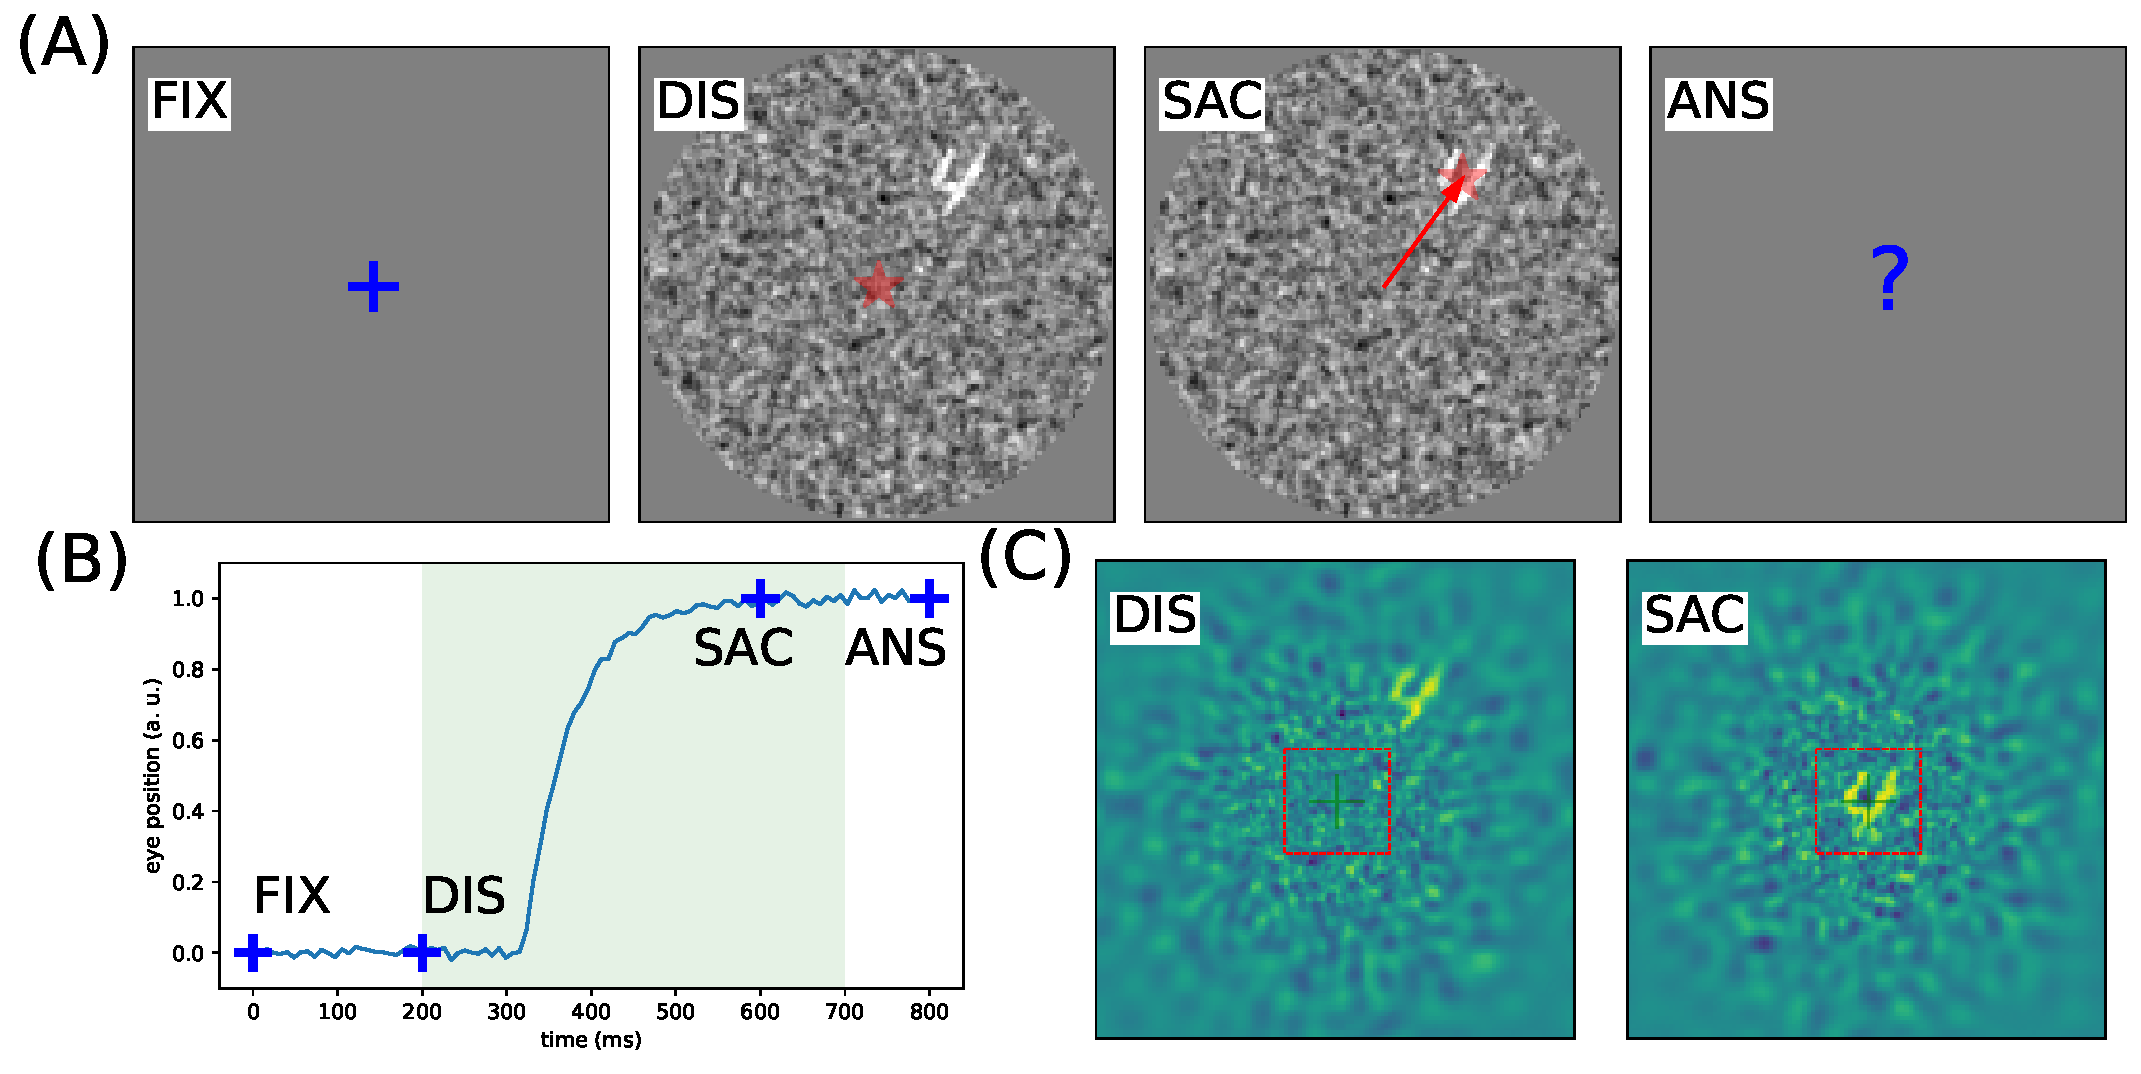
\includegraphics[width=\linewidth]{fig_intro}
	%}
	\caption{
		{\bf Problem setting}: \if 0\CNS In ecological settings, the visual system faces a tricky problem when searching for \emph{any} target in a cluttered environment. It is synthesized in the following experiment:\fi
		(A)~After a fixation period ('FIX') of $200~\ms$, an observer is presented with a luminous display ('DIS') showing a single target from a known class (here digits) and at a random position. The display is presented for a short period of $500~\ms$ (light shaded area in B), that is enough to perform at most one saccade on the potential target ('SAC'). \if 0\CNS In particular, the configuration of the display is such that by adding clutter and reducing the size of the digit it may become necessary to perform a saccade to be able to identify the digit. \fi  Finally, the observer has to identify the digit by a keypress ('ANS'). %
		(B)~Prototypical trace of a saccadic eye movement to the target position. \if 0\CNS In particular, we show the fixation window used to ensure fixation during that window (green shaded area). \fi (C)~Simulated reconstruction of the visual information from the (interoceptive) retinotopic map at the onset of the display ('DIS') and after a (successful) saccade ('SAC'), the dashed red box indicates the visual area of the ``what'' pathway. In contrast to an exteroceptive representation (see A), this demonstrates that the position of the target has to be inferred from this degraded (sampled) image and that a correct identification by the ``what'' pathway is mediated by the action to the location of the target \emph{before seeing it}\if O\CNS , that is before being able to actually be able to identify the target\fi.
		\label{fig:intro}}%
\end{figure}%
%%------------------------------%
The promise of automatic methods to identify objects in natural images is ever increasing. Recently, the performance of such systems outreached the performance of human observers in specific image categorization tasks\if 1\CNS~\citep{He15}\fi. \if 0\CNS Moreover, these systems, which were initially trained on energy greedy, high performance computers, are now designed to work on more common hardware such as desktop computers with a decent GPU~\citep{Sandler18}.
However, such methods are not yet available for mobile devices, as will be necessary for instance for the fast detection of visual objects in autonomous driving, as when one has to distinguish a pedestrian from a sign pole. More importantly, the robustness of such methods is still lower than that of humans. Indeed, it is still difficult for such a system to learn to categorize a particular object class given all the possible spatial configurations and the respective geometrical visual transformations. This explosion of combinations is currently handled by increasing accordingly the number of parameters, hence the energy consumption of such methods. As a consequence, state-of-the art classification architectures contain many millions parameters while still handling relatively small images.

The human visual system, in contrast, is able to perform such a feat very rapidly, in less than 100 ms~\citep{Kirchner06}, and at a low energy cost ($<5~W$). On top of that, this system is mostly autonomous, robust to visual transforms or lighting conditions and can learn with a few examples. If many different anatomical features may explain such efficiency, \fi A main difference of human vision with respect to computer vision lies in the fact that its sensor (the retina) combines a non homogeneous sampling of the world with the capacity to rapidly change its center of fixation. Indeed, on the one hand, the retina is composed of two separate systems: a central, high definition fovea (a disk of about 6 degrees of diameter in visual angle around the center of gaze) and a large, lower definition peripheral area. On the other hand, the retina is attached on the back of the eye which is capable of low latency, high speed eye movements. \if 0\CNS In particular, saccades allow for efficient changes of the position of the center of gaze: They take about $200~\ms$ to initiate, last about $200~\ms$ and usually reach a maximum velocity of approx 600 degrees per second. This behavior is prevalent during our lifetime (about a saccade every 2-3 seconds, that is, almost a billion saccade in a lifetime). \fi The interplay of those two features allows human observers to engage in an action perception loop which sequentially scans and analyses the different parts of the image. 

%It is one type of active inference~\citep{Friston12} (see below) and we will envision herein how to incorporate it to classical computer vision schemes.
% (1 / 2.5 * 3600 * 24 * 365 * 75 = 946080000.0 ~= .95e9) X (wakeful + REM = .66)

To take advantage of this visual behavior, it is of particular importance to understand both its computational and neurophysiological principles.
Active vision methods~\citep{Najemnik05,Butko2010infomax,Friston12}, that provide the ground principles of saccadic exploration, assume the existence of a generative model from which both the target position and identity can be inferred through active sampling. As illustrated in Figure~\ref{fig:intro}-A, inverting a generative model over a large (one-step ahead) hypothesis space of all possible saccades is however computationally-intensive. % (think for instance of face identity as a very large categorical space over a large visual transformation space) with no obvious neurophysiological counterpart.
The goal of this work is to emulate a model of active vision which is able to infer the position of a visual target independently from its identity (but from a known target class), while the position and identity are unknown. This comes with the constraint that the visual sensor is foveated (see Figure~\ref{fig:intro}-C) but can generate a saccade. We will use this constraint as an asset to minimize the overall computational cost of finding a target. This generic visual search problem is of broad general interest in machine learning, computer vision and robotics, but also to neuroscience, as it speaks to the mechanisms underlying foveation and more generally to low-level attention mechanisms. 
\if 0\CNS

\subsection{State of the art}
Several studies are relevant to our endeavor. First, one can consider optimal strategies to solve the problem of the visual search of a target~\citep{Najemnik05}. In a setting similar to that presented in Figure~\ref{fig:intro}-A, where the target is an oriented edge and the background is defined as pink noise, authors show first that a Bayesian ideal observer provides with an optimal strategy, and second that human observers are close to that optimal performance. Though they can predict a sequence of saccades in this perception action loop, this model is limited by the simplicity of the display (elementary edges added on stationary noise and a finite number of locations on a discrete grid) and by the abstract level of modeling. Despite these (inevitable) simplifications, this study could successfully predict some key characteristics of visual scanning such as the trade-off between memory content and rapidity.

Looking more closely at neurophysiology, the study of~\citep{Samonds18} allows to go further in our understanding of the interplay between saccadic behavior and the statistics of the input. In this study, authors were able to manipulate the size of saccades by manipulating key properties of the presented (natural) images. For instance, smaller images generate smaller saccades. Interestingly, they also explained the size of saccades for different species, including mice which lack a foveal region, by the size of visual receptive fields. One key prediction of this study which is relevant for our problem is the fact that saccades seem optimal to \emph{a priori} decorrelate the visual input, that is, to minimize redundancy in the sequence of generated saccades, knowing the statistics of visual inputs.

A further modeling perspective is provided by~\citep{Friston12}. In this model, we first have a full description of the visual world as a generative process, here of the presentation of faces, knowing they are constituted of independent components: mouth, nose, eyes, etc... An agent is completely described by giving the generative model governing the dynamics of its internal beliefs and is interacting with this image by scanning it through a foveated sensor, just as we described in Figure~\ref{fig:intro}. Equipping the agent with the ability to actively sample the visual world enables to explore the idea that actions (saccadic eye movements) are optimal experiments, by which the agent seeks to confirm predictive models of the (hidden) world. One key ingredient to this process is the (internal) representation of counterfactual predictions, that is, of the probable consequences of possible hypothesis as they would be realized into actions (here, saccades).

Such a model constitutes an Active Inference scheme~\citep{Mirza18} and simulations of the resulting optimization scheme reproduce sequential eye movements which fit well with empirical data. Compared to~\citet{Najemnik05}, saccades are not the output of a value-based cost function but a consequence of the seek for the agent to minimize the uncertainty about his beliefs, knowing his priors on the generative model of the visual world. Such an approach applies well to our setting, as described in Figure~\ref{fig:intro}. In particular, we will similarly include a generative process of the visual world as image of a handwritten random digit (drawn from the MNIST database) at a random position and embedded in a cluttered noise. Then, we will equip the agent with a foveated sensor and with the ability to actively scan the visual image as defined by a generative (internal) model. Knowing such priors, we will optimize the behavior of this agent and explore its key properties.

\subsection{Outline}



\fi Stemming from the active vision general principles, our aim is to produce a realistic model that may both explain the essential features of human vision and provide ways toward efficient computer implementations. 

\if 0\CNS
This paper is organized as follows. After this introduction, we will define the notations, variables and equations for the generative process governing the experiment and the generative model for the active vision agent. In particular, we will derive our method to simplify the learning of an optimal agent given these definitions. In section~\ref{sec:results}, we will then show results of numerical simulations of this agent. We will first demonstrate some applications of this framework to different levels of complexity of the problem. This will allow us to derive some limits of this agent and, as in~\citep{Najemnik05}, we will draw some analogies with biologically observed eye movements. Finally, in section~\ref{sec:discussion}, we will summarize these results in comparison with other similar schemes. We will conclude by showing the relative advantages of using this active inference approach.
\fi